\chapter{Introduction}

\section{Cosmic Microwave Background and Inflation}

The observation of the cosmic microwave background (CMB) temperature fluctuations has played a fundamental role in establishing the standard cosmological model, the $\Lambda$ cold dark matter ($\Lambda \mathrm{CDM}$) model, and in constraining key cosmological parameters and the large-scale properties of spacetime. While most of the information about the early Universe has historically been extracted from temperature anisotropies, the polarization of the CMB provides an additional and complementary source of information, offering access to physical processes that are otherwise difficult to probe \cite{2022}.

One of the most important open questions in modern cosmology concerns the origin of the primordial fluctuations that later evolved into the large-scale structure of the Universe. The leading theoretical framework addressing this question is cosmic inflation, a period of accelerated expansion occurring at very early times. During inflation, microscopic quantum fluctuations were stretched to macroscopic scales, seeding both density perturbations and tensor perturbations in the spacetime metric. These initial fluctuations eventually gave rise to galaxies, clusters, and the cosmic web observed today.

\begin{figure}[htbp]
    \centering
    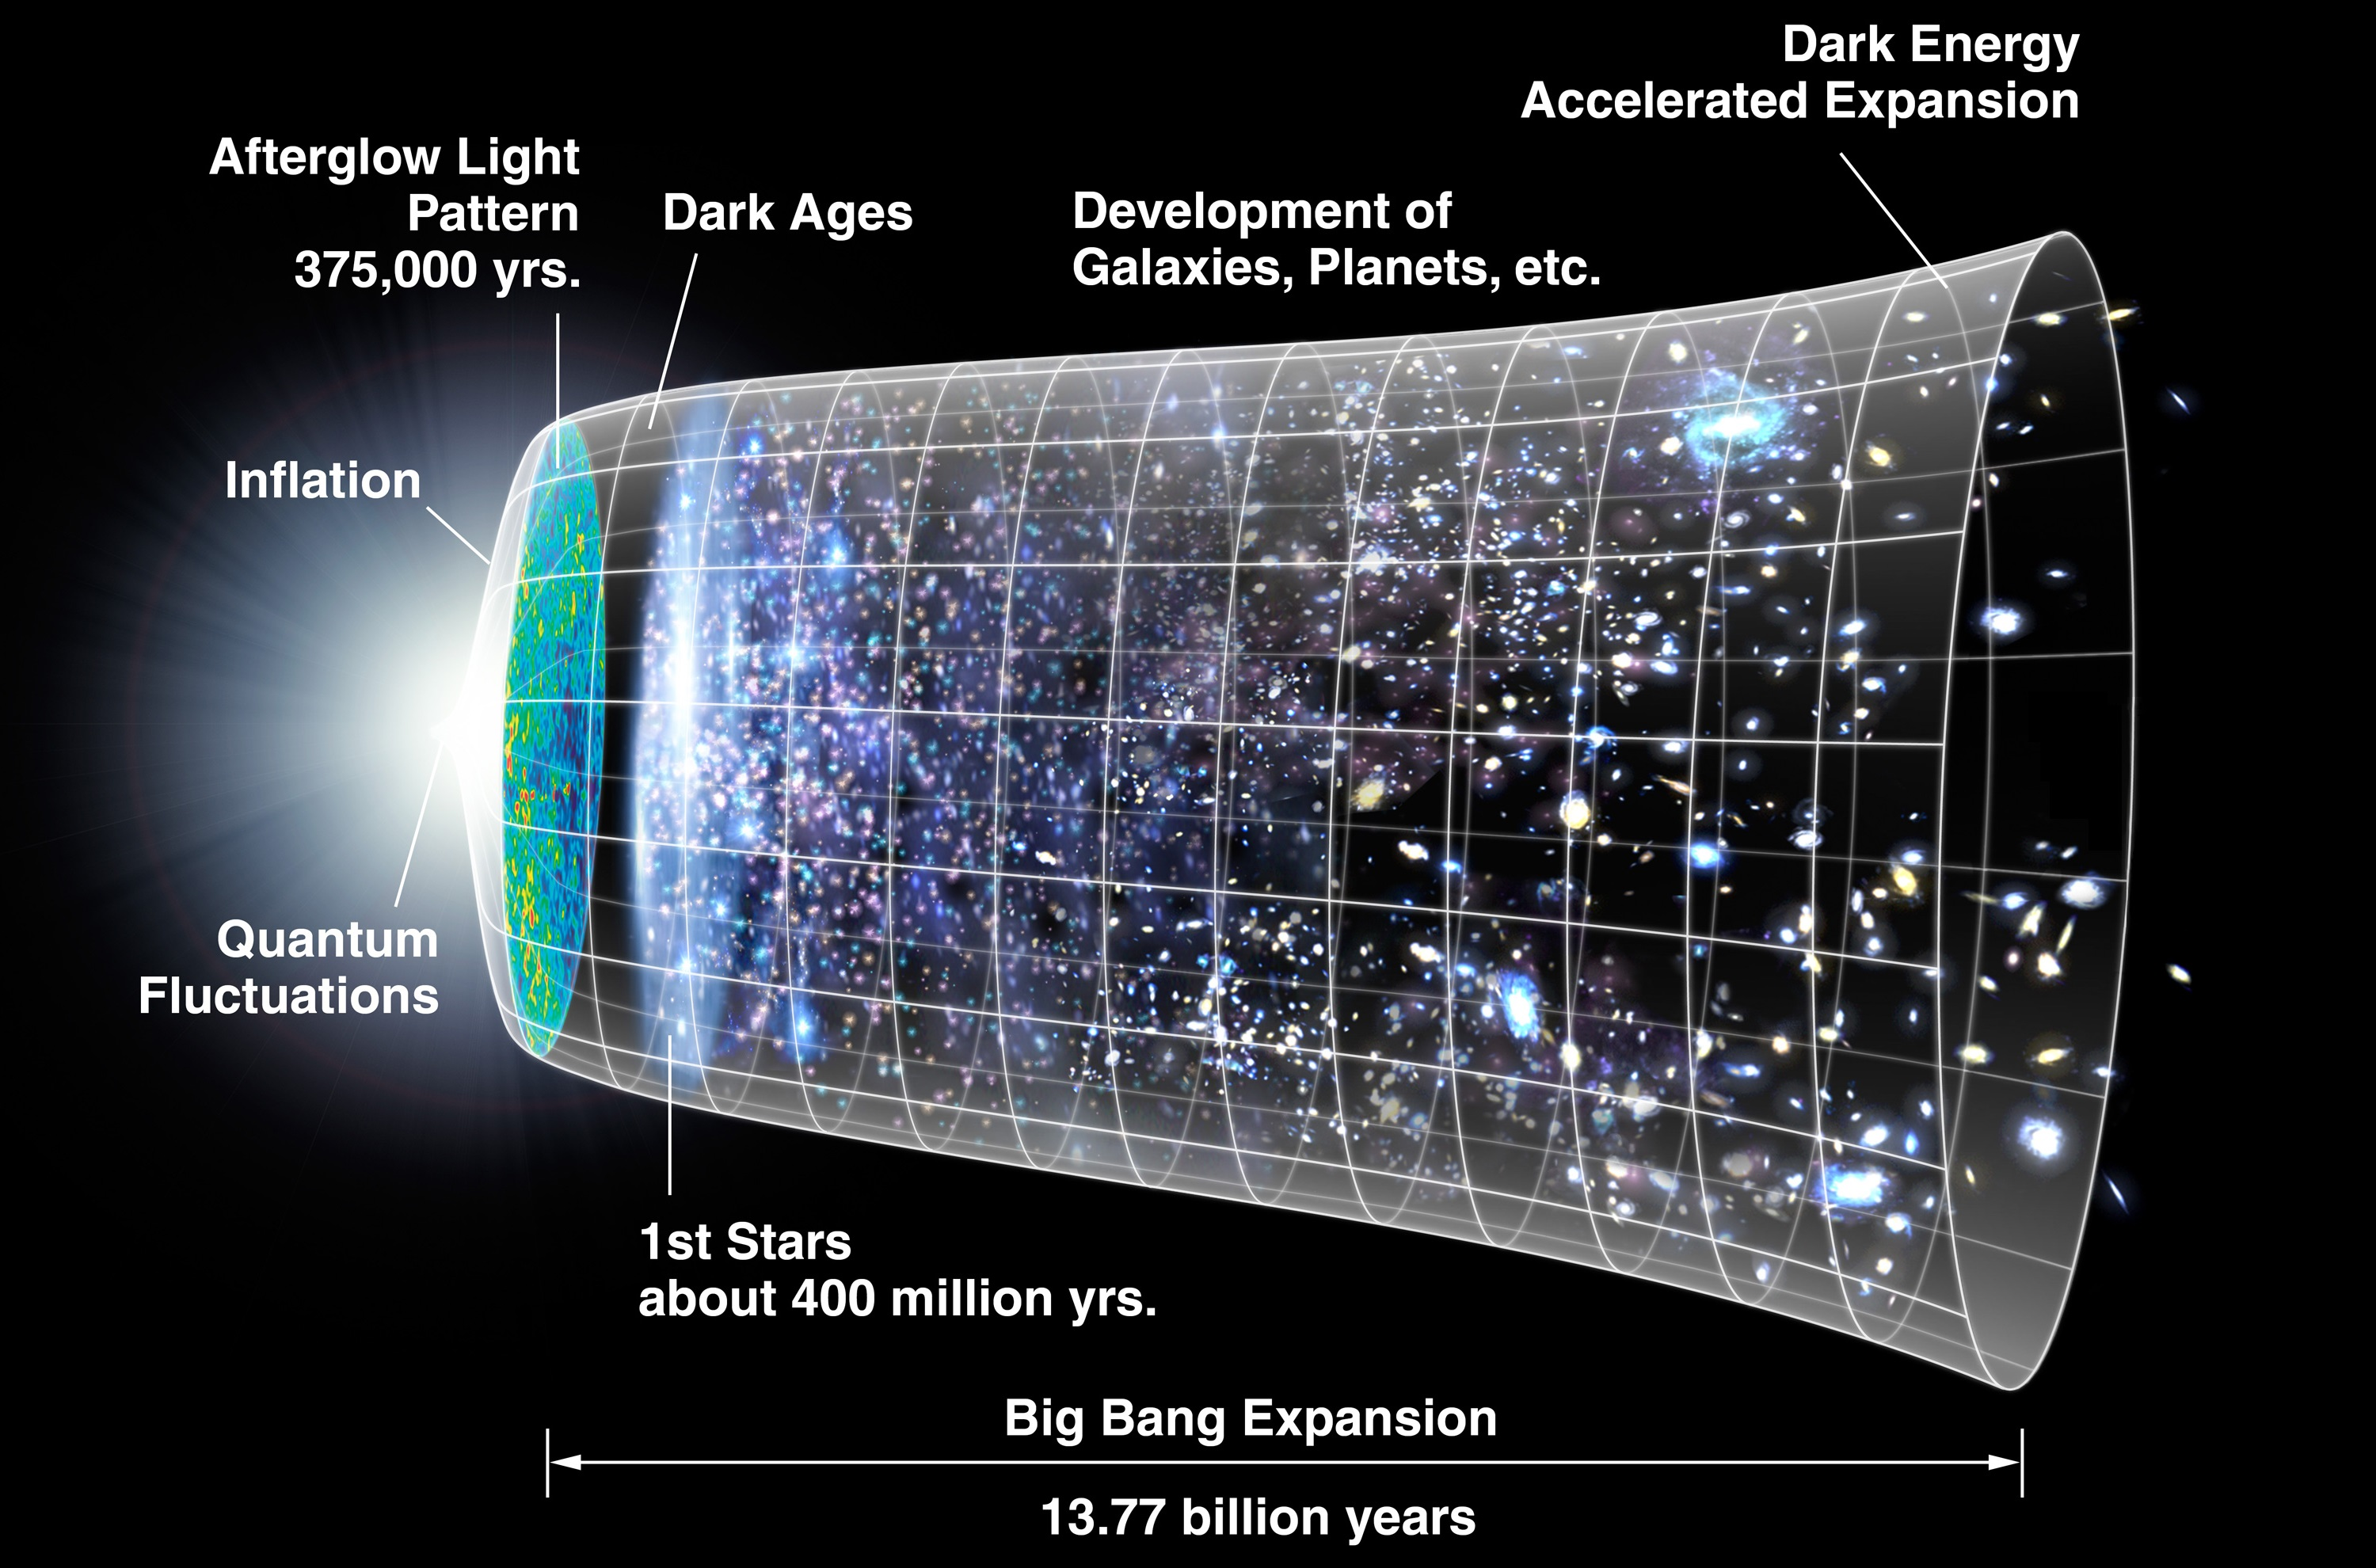
\includegraphics[width=0.7\textwidth]{1_bigbang_expansion}
    \caption{Timeline of the Universe according to the standard cosmological model. The diagram illustrates the expansion from the initial quantum fluctuations, through the epoch of inflation, to the emission of the CMB approximately 375,000 years after the Big Bang, and finally the subsequent formation of large-scale structures.}
    \label{fig:universe_timeline}
\end{figure}

Inflation predicts not only the scalar perturbations responsible for CMB temperature anisotropies, but also a stochastic background of primordial gravitational waves. While scalar perturbations dominate the temperature signal, tensor perturbations leave a characteristic imprint in the polarization of the CMB, providing a unique observational window onto the inflationary epoch. Detecting such a signal would offer direct evidence for inflation and allow access to energy scales far beyond the reach of terrestrial experiments \cite{2022}.



\section{CMB Polarization and Primordial \textit{B}-Modes}

The polarization of the CMB arises from Thomson scattering of photons in the presence of local quadrupole temperature anisotropies at the surface of last scattering and during the epoch of reionization. The polarization pattern on the sky can be decomposed into two components, known as \textit{E}-modes and \textit{B}-modes, which differ in their symmetry properties under parity transformations.

\textit{E}-mode polarization is primarily generated by scalar density perturbations and has been robustly detected by several experiments. \textit{B}-mode polarization, on the other hand, is of particular interest because it can be sourced by tensor perturbations, such as primordial gravitational waves produced during inflation. Since scalar perturbations do not generate \textit{B}-modes at linear order, the detection of a primordial \textit{B}-mode signal would constitute a distinctive signature of inflationary physics.

\begin{figure}[htbp]
    \centering
    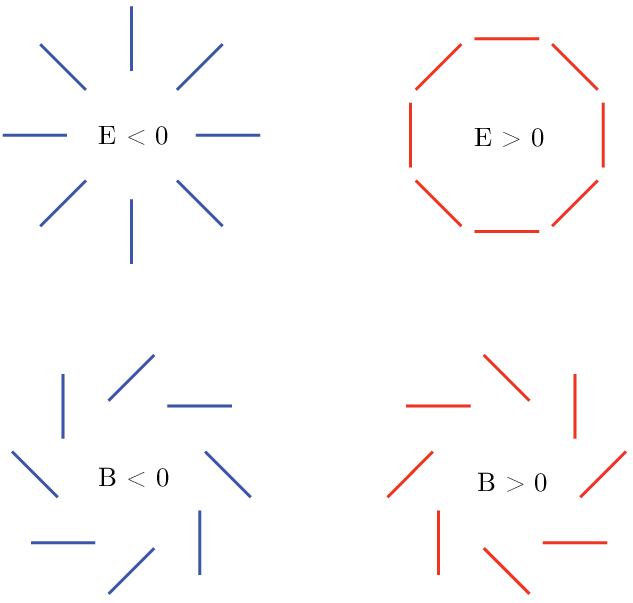
\includegraphics[width=0.38\textwidth]{1_eb_modes.png}
    \caption{Schematic representation of CMB polarization modes. Top: $E$-modes exhibit a curl-free, symmetric pattern under parity transformation ($E > 0$ for tangential, $E < 0$ for radial). Bottom: $B$-modes exhibit a divergence-free, spiral pattern, changing sign under parity reflection.}
    \label{fig:eb_modes}
\end{figure}

In addition to a possible primordial contribution, \textit{B}-modes can also be generated through secondary effects. Gravitational lensing by large-scale structures distorts the polarization field, converting part of the \textit{E}-mode signal into \textit{B}-modes, while Galactic foreground emissions further contaminate the observed signal. Disentangling the primordial component therefore requires high sensitivity, broad frequency coverage, and careful control of instrumental and observational systematics.



\section{The LiteBIRD Mission}

\textit{LiteBIRD (Lite \textit{B}-mode polarization and Inflation from cosmic background Radiation Detection)} is a space mission dedicated to primordial cosmology and fundamental physics. Its primary scientific goal is the detection of polarization from primordial gravitational waves, which would provide direct evidence for cosmic inflation and probe physics at energy scales far beyond those accessible on Earth \cite{2022}.

LiteBIRD will operate at the Sun--Earth Lagrange point L2, a stable environment that enables continuous full-sky observations with minimal contamination from the Earth, Moon, and Sun. From this orbit, the satellite will survey the CMB polarization over a nominal mission duration of three years.

The mission observes the sky in 15 frequency bands from 34 to 448~GHz, allowing efficient separation of the primordial CMB signal from Galactic and extragalactic foregrounds. LiteBIRD aims for an unprecedented total sensitivity of approximately 
$2.2~\mu\mathrm{K \cdot arcmin}$, with a typical angular resolution of about 
$0.5^\circ$ at 100~GHz, as reported in \cite{2022}. This makes it complementary to ground-based experiments, which generally target smaller sky areas, whereas LiteBIRD focuses on the largest angular scales through full-sky coverage.

A key scientific requirement is to reach a sensitivity sufficient to detect the primordial gravitational wave amplitude, expressed in terms of the tensor-to-scalar ratio $r$\footnote{
The tensor-to-scalar ratio $r$ quantifies the relative amplitude of primordial tensor perturbations (gravitational waves) with respect to scalar perturbations (density fluctuations) generated during inflation. It is defined as the ratio between the power spectra of tensor and scalar modes,
\[
r \equiv \frac{\Delta_h^2(k)}{\Delta_\zeta^2(k)} = \frac{A_t}{A_s},
\]
where $\Delta_h^2(k)$ and $\Delta_\zeta^2(k)$ denote the dimensionless tensor and scalar power spectra, and $A_t$ and $A_s$ are their corresponding amplitudes evaluated at a given pivot scale $k$. A detection of a non-zero value of $r$ would provide direct evidence for primordial gravitational waves and strongly support the inflationary paradigm.
}. LiteBIRD aims for a total uncertainty $\delta r < 10^{-3}$, enabling either detection of primordial \textit{B}-modes or stringent constraints on inflationary models. In particular, it targets both the recombination peak ($\ell \simeq 80$) and the reionization peak ($\ell \lesssim 10$) in the \textit{B}-mode power spectrum, which together would provide robust evidence for an inflationary origin.

\begin{figure}[htbp]
    \centering
    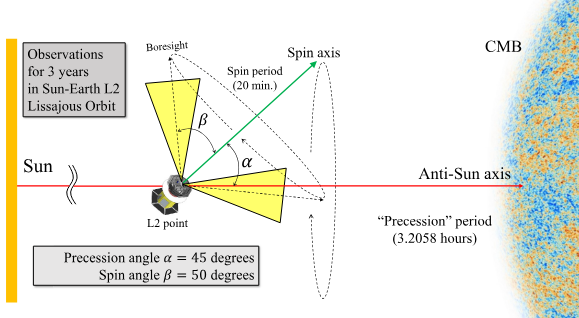
\includegraphics[width=0.8\textwidth]{1_satellite.png}
    \caption{The telescope boresight is at an angle $\beta = 50^{\circ}$ to the spin axis and rotates at a rate of $0.05$\,rpm. The spin axis is rotated around the anti-Sun direction through precession with an angle $\alpha = 45^{\circ}$ in $3.2058$\,h. The anti-Sun axis rotates around the Sun in one year. With a combination of the three motions, the boresight can cover the entire sky in half a year. (Image adapted from \cite{2022}).}
    \label{fig:litebird_scan}
\end{figure}

The payload comprises three telescopes covering complementary frequency ranges: the Low-Frequency Telescope (LFT), the Mid-Frequency Telescope (MFT), and the High-Frequency Telescope (HFT). Multichroic detectors allow each pixel to observe multiple frequency bands, maximizing sensitivity while keeping the focal plane compact.

LiteBIRD scans the sky using a combination of continuous rotation around its own axis, slow precession around the Sun–Earth direction, and annual revolution around the Sun. This scanning strategy ensures uniform sky coverage, high redundancy in polarization angle sampling, and suppression of systematic effects. A continuously rotating half-wave plate modulates the polarization signal, reducing low-frequency ($1/f$) noise and instrumental systematics. Thermal and mechanical stability of the spacecraft further minimize noise contributions.

Access to the largest angular scales, particularly the reionization \textit{B}-mode signal, is uniquely achievable from space. Correlated low-frequency noise and long-term drifts can significantly affect these measurements, making accurate instrumental noise modeling critical for assessing LiteBIRD's sensitivity and scientific performance.



\section{Aim and Structure of the Thesis}
The main objective of this thesis is the simulation and comparison of instrumental noise models for the LiteBIRD mission, focusing on white noise and correlated $1/f$ noise, which dominate in large-angular-scale CMB polarization experiments.

The work uses the LiteBIRD Simulation Framework (LBS), a Python-based simulation 
package for modeling the data acquisition of LiteBIRD instruments, as presented 
in \cite{Tomasi2025}, along with the \texttt{ducc0} numerical library\footnote{\url{https://gitlab.mpcdf.mpg.de/mtr/ducc}} 
by Martin Reinecke for efficient numerical computation. In this work, two new noise-addition functions have been implemented to operate 
block-wise, enabling long-duration simulations while controlling memory usage. 
These functions are based on pre-existing noise-generation routines: one provided by the LiteBIRD Simulation Framework and one by the \texttt{ducc0} library.

The two noise models are validated and compared in both time and frequency domains. Time-domain signals and power spectral densities are examined to verify agreement with theoretical expectations, while noise-only sky maps and hit maps assess the impact of correlated noise on large angular scales. Performance is also evaluated in terms of computational time and memory usage, with attention to optimization strategies for long-term simulations.

This thesis is organized as follows. Chapter~2 provides the scientific background on instrumental noise in CMB experiments, detailing white and $1/f$ noise, power spectral density, and HEALPix sky pixelization. Chapter~3 describes the simulation framework, the scanning strategy, and the detector models adopted for LiteBIRD. Chapter~4 presents the noise generation strategy and the technical implementation of the two block-wise models. Chapter~5 focuses on the validation of the models through time-domain and frequency-domain analyses. Chapter~6 extends the analysis to long-term simulations, map-making, and the estimation of the angular power spectrum for temperature ($C_\ell^{TT}$). Finally, Chapter~7 summarizes the results obtained and discusses potential future developments.
